\section{Motivation}

\begin{frame}[t]{Welcome to CNNs!}
    \textbf{Topic: Introduction to Convolution and CNNs}

    \vspace{1em}
    \textbf{What we’ll learn today:}
    \begin{itemize}
        \item How computers see images
        \item What is convolution
        \item How CNNs work
        \item Implementing CNNs in PyTorch
    \end{itemize}
\end{frame}

\begin{frame}[allowframebreaks]{Motivation}
    \begin{figure}
        \centering
        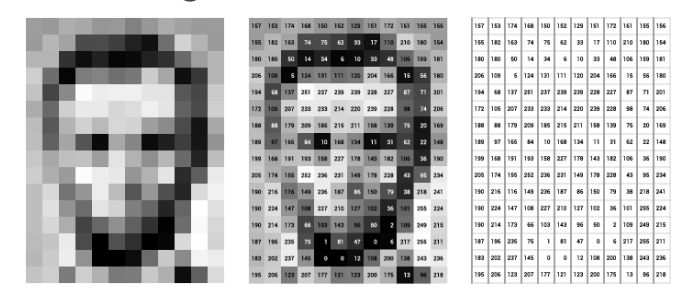
\includegraphics[height=0.9\textheight,width=1\textwidth,keepaspectratio]{images/cnn/represent_image.png}
    \end{figure}

    \begin{itemize}
        \item Humans are amazing at understanding images: recognizing faces, reading signs, identifying objects.
        \item Computers? Not so much. They need help!
    \end{itemize}

    \framebreak

    \begin{figure}
        \centering
        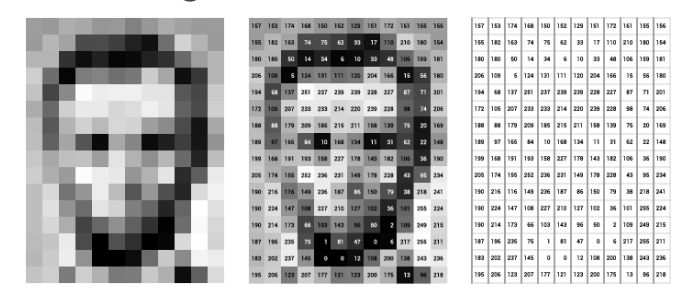
\includegraphics[height=0.8\textheight,width=0.8\textwidth,keepaspectratio]{images/cnn/represent_image.png}
    \end{figure}

    \begin{itemize}
        \item What we human see as a simple image is just a grid (or matrix) of numbers to a computer.
        \item Each pixel has a value (0-255 for grayscale, 3 values for RGB).
        \item Computers need to learn patterns in these numbers to understand images.
        \framebreak
        \item \large Convolution and CNNs are the backbone of modern computer vision.
        \item Used in self-driving cars, medical diagnosis, facial recognition, etc.
    \end{itemize}
\end{frame}

\begin{frame}[allowframebreaks]{Some Applications}

    \foreach \i in {2,...,13} { % Integers from 1 to 5
        \begin{figure}
            \centering
            \includegraphics[height=0.9\textheight,width=1\textwidth,keepaspectratio]{images/cnn/cv_\i.png}
        \end{figure}

        \framebreak
    }

    % \begin{figure}
    %     \centering
    %     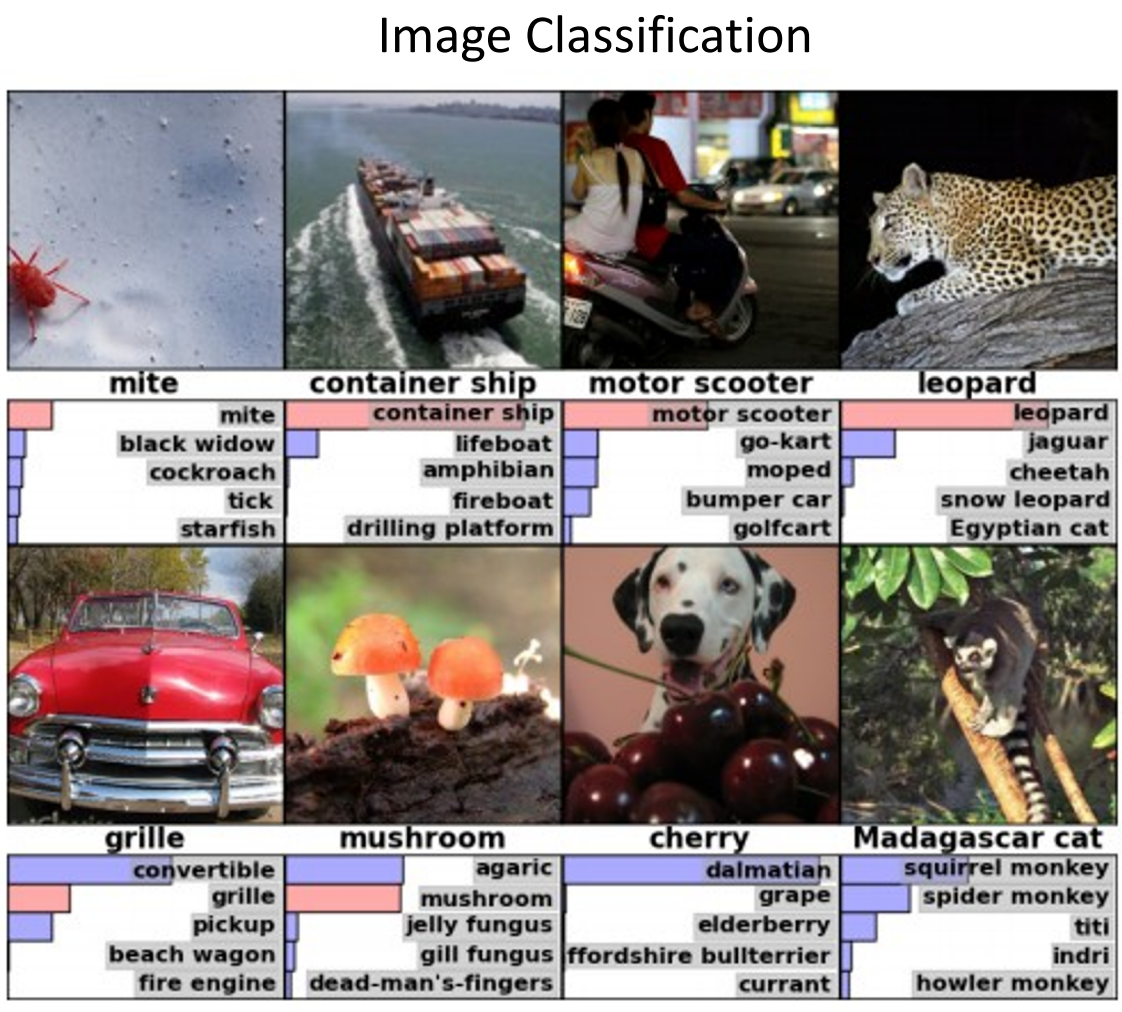
\includegraphics[height=0.9\textheight,width=1\textwidth,keepaspectratio]{images/cnn/cv_2.png}
    % \end{figure}

    % \framebreak

    % \begin{figure}
    %     \centering
    %     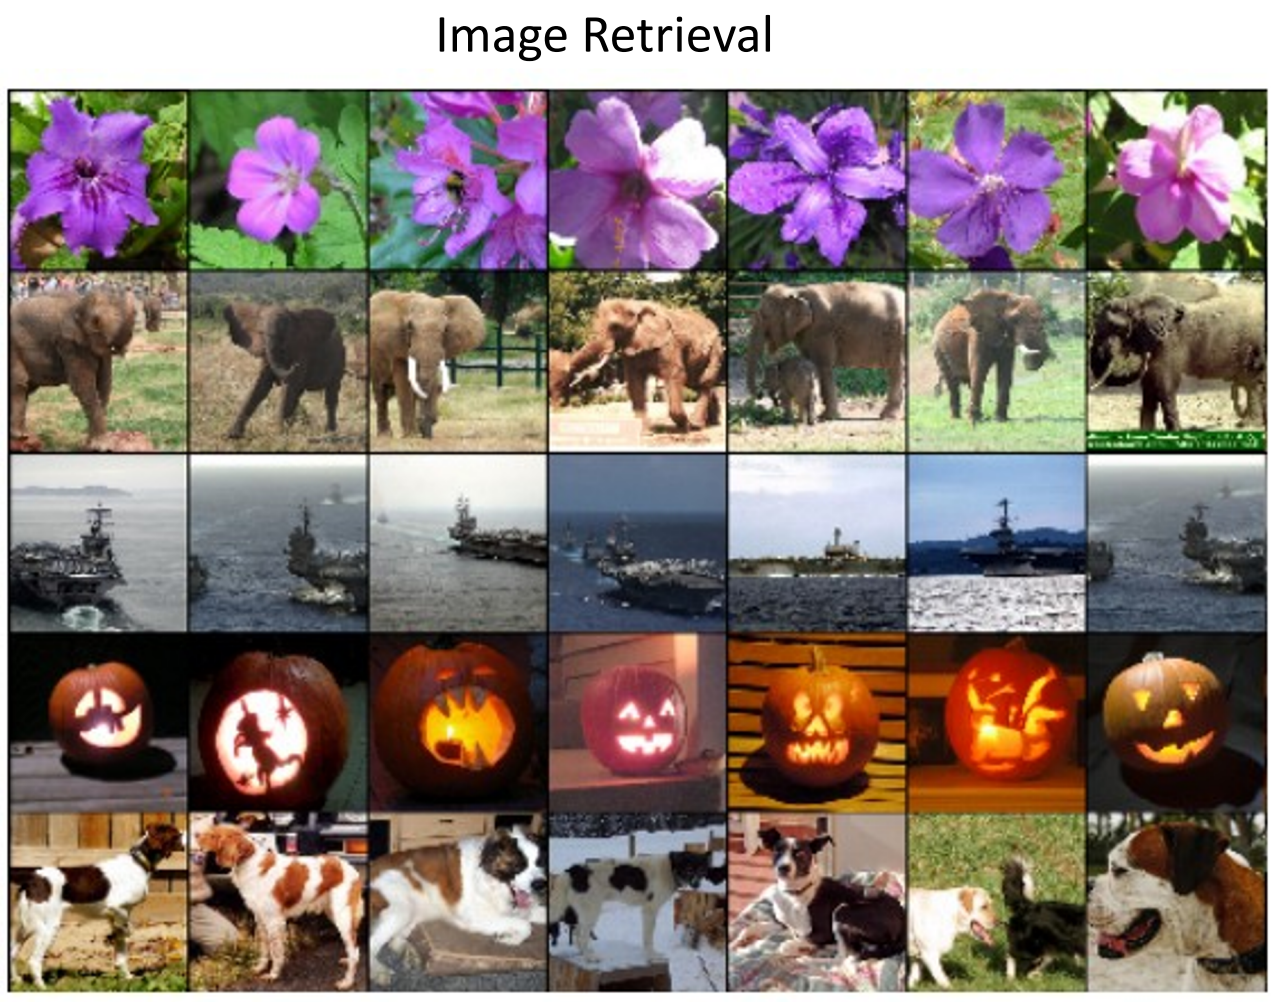
\includegraphics[height=0.9\textheight,width=1\textwidth,keepaspectratio]{images/cnn/cv_3.png}
    % \end{figure}

    % \framebreak

    % \begin{figure}
    %     \centering
    %     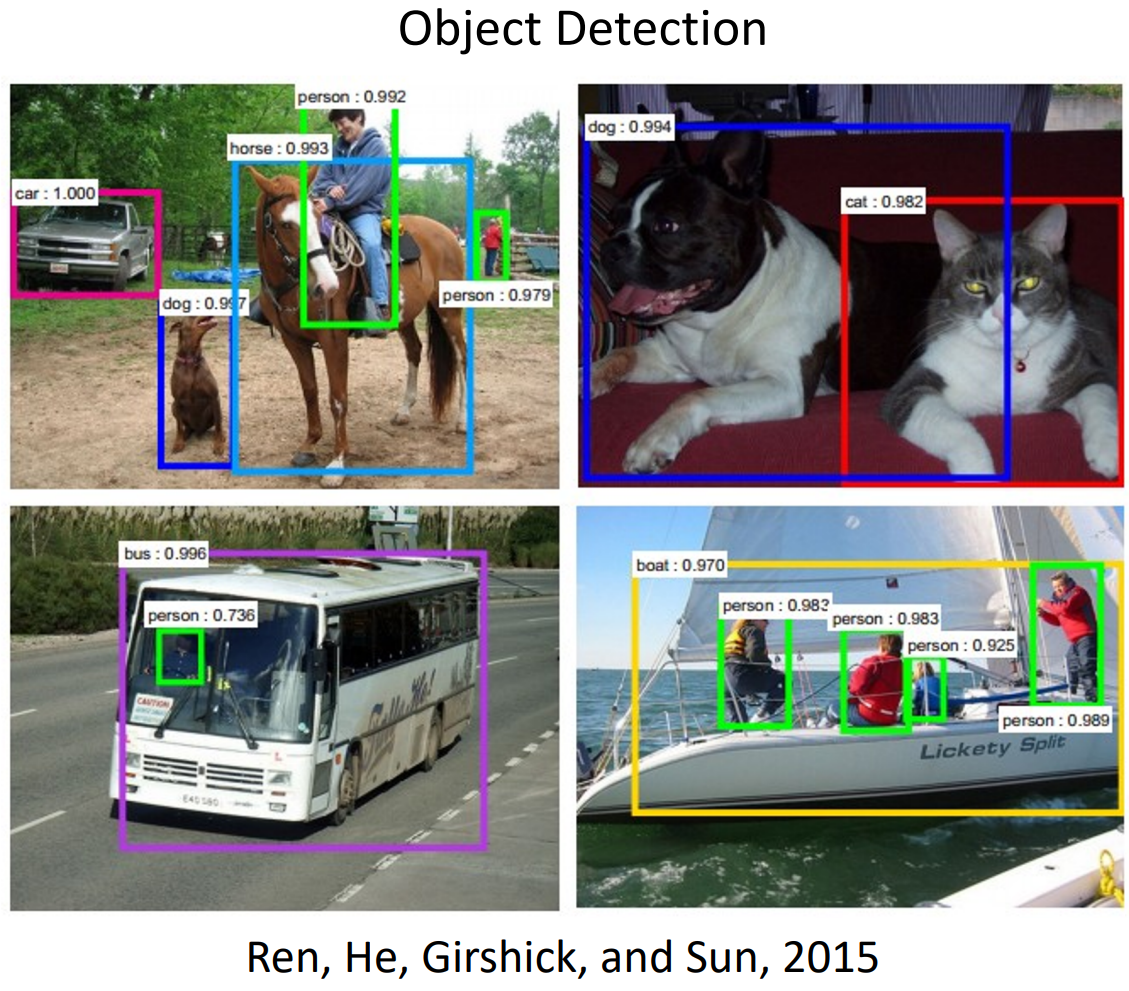
\includegraphics[height=0.8\textheight,width=1\textwidth,keepaspectratio]{images/cnn/cv_4.png}
    % \end{figure}

    % \framebreak

    % \begin{figure}
    %     \centering
    %     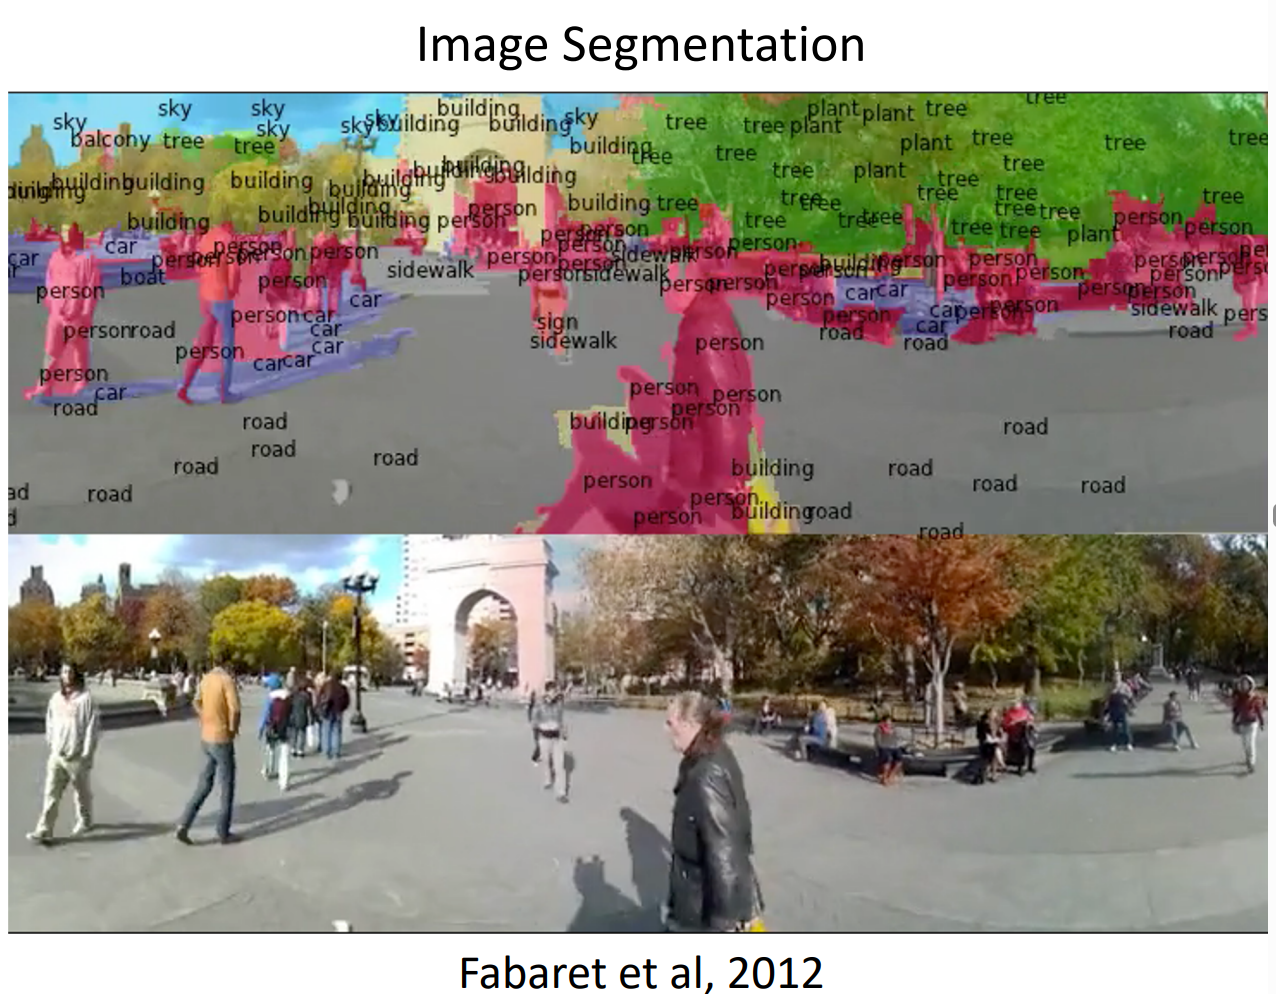
\includegraphics[height=0.8\textheight,width=1\textwidth,keepaspectratio]{images/cnn/cv_5.png}
    % \end{figure}

    % \framebreak
\end{frame}

\begin{frame}[allowframebreaks]{Motivation}
    \begin{itemize}
        \item \textbf{Transformative Impact:} Convolutional Neural Networks (CNNs) have revolutionized computer vision and deep learning.
        \item \textbf{Wide Applications:} Power tasks such as image classification, object detection, facial recognition, and medical image analysis.
        \item \textbf{Automatic Feature Learning:} CNNs learn hierarchical features directly from raw pixel data, reducing the need for manual feature engineering.
        \item \textbf{Demystifying CNNs:} This presentation breaks down core components and traces the evolution of key architectures.
        \item \textbf{Practical Relevance:} Understanding CNNs enables better design, optimization, and application to real-world problems.
    \end{itemize}
\end{frame}